%Préambule du document :
\documentclass[12pt, a4paper]{book}
%\usepackage[latin1]{inputenc} 
\usepackage[utf8]{inputenc} % accents
\usepackage{gensymb} % degree symbol ° (\degree)
\usepackage[T1]{fontenc} % | "`pipe"' character
\usepackage{graphicx}
\usepackage{titling}
\usepackage{amssymb} 
\usepackage{minitoc} % chapter's tocs
\usepackage{authblk} % author affiliations
\usepackage{fancyhdr} % modify the headers
\usepackage{tabularx} % tables not larger than A4
\usepackage[table]{xcolor} %colors inside the tables
\usepackage{float}
\usepackage{multicol} % multiple columns in some sections
\usepackage[inner=2cm,outer=2cm]{geometry} %A4 margins
\usepackage{siunitx}
\usepackage[labelfont=bf, margin=0.5cm]{caption} % for figure captions in minipages
\usepackage{hyperref} %link references (toc, citations) inside document
\usepackage{natbib} % to cite with parentheses and plain text et only year if you please...
\usepackage{amsmath}
 \usepackage{fixltx2e} % allows overrightarrow to be in caption
 \MakeRobust{\overrightarrow}




\bibliographystyle{plainnat} % reference style
\renewcommand{\bibname}{References} %Rename "`bibliography"' => "`references"'

\hypersetup{
    colorlinks,
    citecolor=brown,
    filecolor=green,
    linkcolor=red,
    urlcolor=blue
}
\hypersetup{linktocpage}


\pagestyle{fancy}
\fancyhead{}
\fancyfoot{}
\fancyhead[RO,LE]{\thepage}
\fancyhead[LO]{\leftmark}
\fancyhead[RE]{\rightmark}
\setcounter{tocdepth}{1} % we only want chapters and sections in toc
\setcounter{minitocdepth}{2} %we want sections and subsections in chapters' minitocs

\pretitle{%
  \begin{center}
  
  
\includegraphics[width=17cm]{../Logo_software.png}\\[\bigskipamount]
}
\posttitle{
\\
  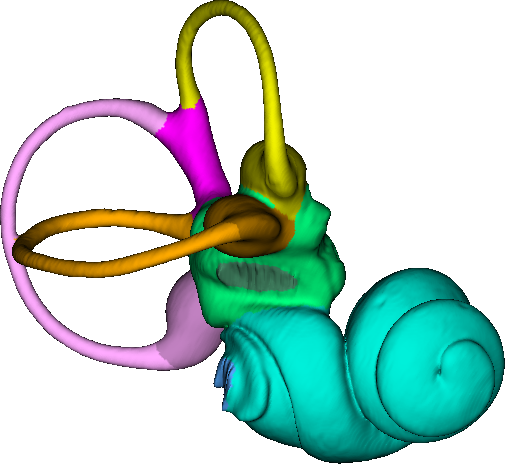
\includegraphics[width=6.5cm]{tutorial05.png}\\[\bigskipamount]
\end{center}}

%\postdate{
%
\includegraphics[width=15cm]{logo_affiliations.png}
%}

\title{Tutorial 02: working with curves}



%\titlepicture[width=13cm]{Logo_software.png}
\author{Renaud LEBRUN}
\affil{Institut des Sciences de l'Evolution, Université de Montpellier, France}
\date{\today} 

\def\chaptername{Tutorial}
\setcounter{chapter}{5}
%Corps du document :
\begin{document}

\dominitoc	

\maketitle

\faketableofcontents

\addstarredchapter{Working with tags}

\markboth{Tutorial 05: Working with tags}{}

\minitoc 
Tutorial 02 includes:
\begin{itemize}
\item One .ntw (MorphoDig project) file
\item One .vtk surface file representing a right inner ear of \textit{Galago moholi}
\item One .pos (position) file 
\item One .ori (orientation helper labels) file 
\item One .tgp (tag map) file
\item The present .pdf document
\end{itemize}





\section{About the specimen}

%\addcontentsline{toc}{section}{About the specimen}
The surface file enclosed in this tutorial represent three-dimensional reconstruction of the right inner ear of a strepsirrhine primate (\textit{Galago moholi}) obtained by computerized microtomography at the MRI \si{\micro} CT.\\
Before using this tutorial, please download and read MorphoDig User Guide.


\section{A brief overview of enclosed files}
		Download and unzip the files associated to this tutorial. Open MorphoDig.
\subsection{Mouse inner ear surface and position files}
	You may open the enclosed .vtk surface file (File -> Surface -> Open Surface, then select "Galago\_moholi\_right\_ear.vtk", or drag and drop this file in the 3D main window). When opened
this way, the corresponding opened surface object is drawn grey, which indicates that this surface
is selected. You may interact with selected objects in different ways (see MorphoDig user guide for
further explanations).\\


By default (\includegraphics[scale=0.7]{../images/06/camera/move_cam2.png}), the camera rotates around the center of mass of all opened objects. This behavior is useful when the center of mass of an object (or of several ones) is far from the origin of the coordinate system. But by pressing the camera button (\includegraphics[scale=0.7]{../images/06/camera/move_cam2.png} -> 
\includegraphics[scale=0.7]{../images/06/camera/move_cam.png}), the camera will revolve around the center of the coordinate system (x=0, y=0, z=0).  The display grid is drawn using different colors depending on the camera rotation center (see Fig. \ref{grid_color} p.\pageref{grid_color}).



 As a general rule, when opening a new surface, it is strongly advised to change its position in order that it matches the 6 predefined camera positions :\\

\includegraphics[scale=0.7]{../images/06/camera/camera_right.png} view object from right side \\

\includegraphics[scale=0.7]{../images/06/camera/camera_left.png} view object from left side\\

\includegraphics[scale=0.7]{../images/06/camera/camera_front.png} view object from front side (default camera position)\\

\includegraphics[scale=0.7]{../images/06/camera/camera_back.png} view object from back side\\

\includegraphics[scale=0.7]{../images/06/camera/camera_above.png} view object from above\\

\includegraphics[scale=0.7]{../images/06/camera/camera_below.png} view object from below\\

In "object interaction mode(
\includegraphics[scale=0.7]{../images/04/move_mode.png})", selected objects can be translated and rotated using the mouse left and middle buttons (in landmark 
\includegraphics[scale=0.7]{../images/04/Landmarks2.png} and camera  
\includegraphics[scale=0.7]{../images/04/camera_mode.png} selection modes, you also need to maintain ``CTRL" button pressed while dragging the left mouse button to achieve rotation and translation of selected objects). Alternatively, you may also use the "yellow sliders" located on the right side of the 3D main window to accomplish rotation and translation of selected objects. Rotation is achieved around the global center of mass of all currently selected objects.\\
\begin{figure}
  \centering
  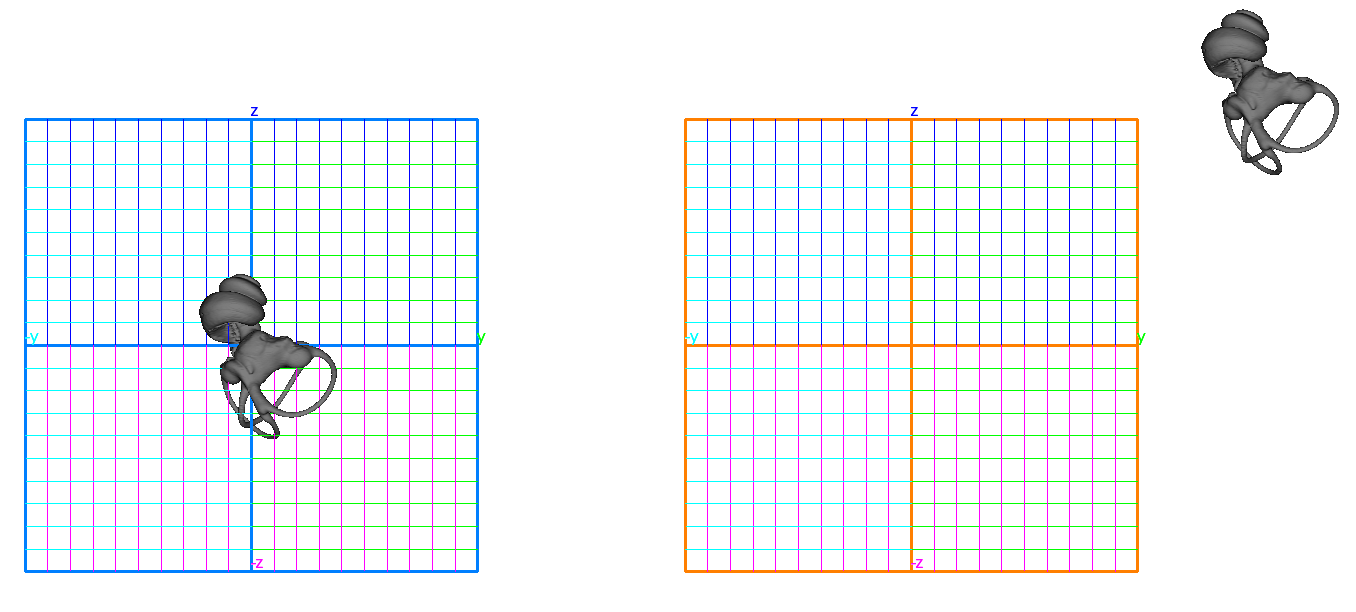
\includegraphics[scale=0.3]{grid.png} 
	\caption{Grid display color.  Left: when the camera revolves around the center of mass of all opened objects, the grid has a blue outline. Right: when the camera revolves around the origin of the coordinate system (x=0, y=0, z=0), the grid outline is displayed in orange.}
\label{grid_color}
 
\end{figure}

A convenient way to orient a right inner ear in a biologically relevant way is done as follows (see Fig. \ref{orientation} p.\pageref{orientation}):\\
1) place camera to view object from the front side (
\includegraphics[scale=0.7]{../images/06/camera/camera_front.png})\\
2) place the lateral semi-circular canal in the horizontal plane (x-y plane)\\
3) place camera  to view object from above ( 
\includegraphics[scale=0.7]{../images/06/camera/camera_above.png} )\\
4) rotate the inner around the z axis ("rz" yellow slider) until the later semicircular points towards the top left-hand part of the screen, and the cochlea points towards the bottom right-hand of the screen.\\
That way, when viewing the inner ear from the front side (
\includegraphics[scale=0.7]{../images/06/camera/camera_front.png}), it is approximately oriented in the same way as it would be within the cranium viewed from the front side as well.\\

The present tutorial contains a .pos (position) file, which you may open in order to place correctly the right ear of the \textit{Galago moholi} (File -> Position-> Open Position for selected surfaces, then choose "Galago\_moholi\_right\_ear.pos", see Fig. \ref{orientation} p.\pageref{orientation}). As we plan to place curve node landmarks and curve handle landmarks inside the cochlea and the semicircular canals, please select the right inner ear surface (CTRL+A, or drag right mouse button to draw a selection rectangle) and change its transparency (Edit Selected Surface->rendering modifications->Change transparency -> then give a value smaller than 100).\\
All opened surfaces can be unselected by pressing "CTRL +D", or selected by pressing "CTRL +A". All selected objects can be deleted by pressing "Del".

\begin{figure}
  \centering
  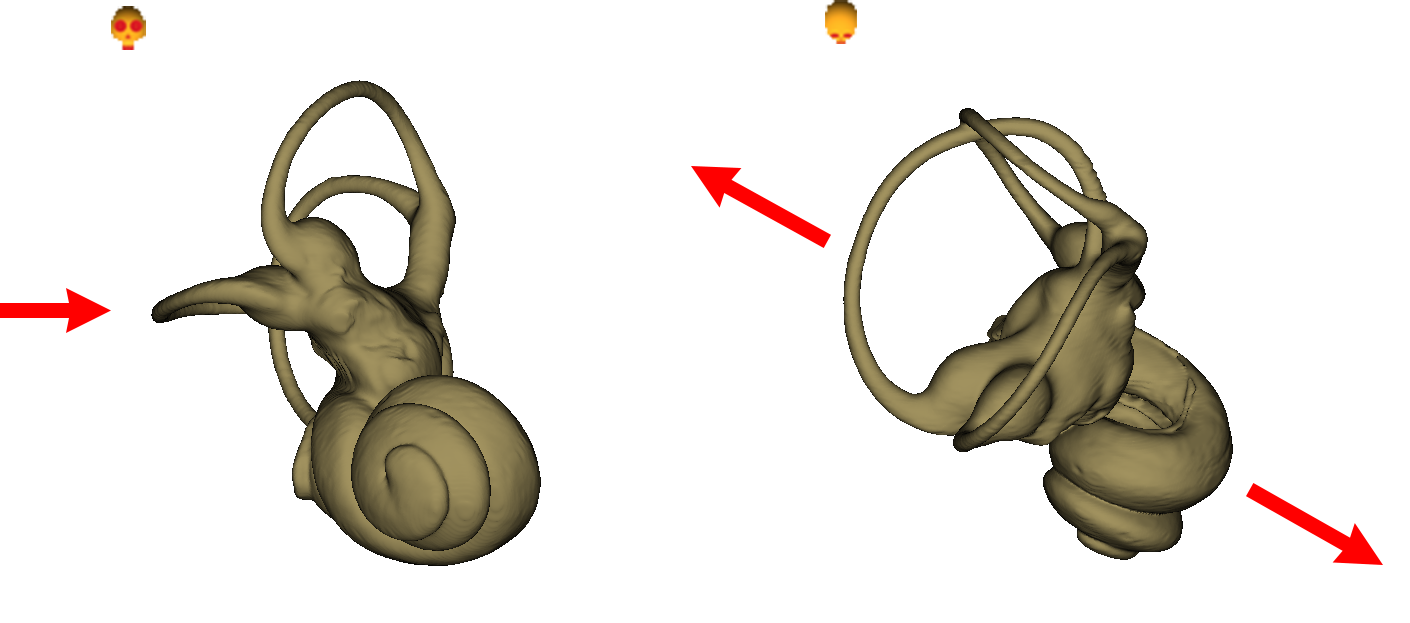
\includegraphics[scale=0.3]{pos.png} 
	\caption{A convenient way to orientate right inner ears.  Left: when viewed from the front side, the lateral canal is placed horizontally. Right: when viewed from above, the cochlea points towards the bottom right-hand of the screen, and the lateral canal towards the top left-hand of the screen.}
\label{orientation}
 
\end{figure}


\subsection{Galago moholi inner ear project file}
The present tutorial contains a project .ntw file, which may be useful to directly open the right inner ear
 in a convenient position, to make it transparent and to give it a color. First, delete all currently opened objects
(press "CTRL+A", then press "Del"). Then open the enclosed .ntw file (File -> Open Project, then select
"Galago\_moholi\_right\_ear.ntw"). Once loaded, the right inner ear surface is opened, is given the position
enclosed in the "Galago\_moholi\_right\_ear.pos" file, a color and a transparency. Note that the newly opened
surface is unselected.\\

\subsection{Galago moholi tag map file}
3D Curves are constructed in MorphoDig using 2 series of landmarks : a series of "curve node" landmarks (
\includegraphics[scale=0.7]{../images/04/curve_nodes.png}),
and a series of "curve handle" landmarks (
\includegraphics[scale=0.7]{../images/04/curve_handles.png}). The numbers of curve nodes and curve handles should be equal. The Galago\_moholi\_right\_ear.stv contains the 3D coordinate of a series of  33 "curve node" and 33 "curve handle" landmarks. You can load it (File->Curves->Load MorphoDig Landmark/Curve file(.STV), or drag and drop this file directly in the 3D main window).\\

You may consider to change the way landmarks and curve handles are rendered in the "Landmark and flag options" window (Edit->Edit landmark and flag rendering options ). In this tutorial, you may display landmarks as spheres and to set their rendering size to 0.05 mm.\\

\subsection{Galago moholi inner ear .ori file}
The present tutorial contains a .ori file, which contains orientation labels for the coordinate system
orientation helper. You can load this file the enclosed .ori file ("File->Orientation helper labels -> Open Orientation labels", then select
"Galago\_moholi\_right\_ear.ori"). Once loaded, the system coordinate orientation helper will show the following
labels :\\
+z axis : superior\\
-z axis : inferior\\
+y axis : medial\\
-y axis : lateral\\
+x axis : proximal\\
-x axis : distal\\
You may set your own orientation axis labels with the “Edit orientation labels” window (Edit-> Edit orientation labels)

\section{Curve digitization with MorphoDig}


When digitizing curve node and curve handle landmarks, I recommend to press "
\includegraphics[scale=0.7]{../images/04/Landmarks2.png}" to activate the "Landmark mode". When active, only landmarks can be selected/unselected via right mouse button drag/click. \\

As stated earlier, two series of landmarks involved into the construction of 3D curves can be set with MorphoDig: "curve node" and "curve handle" landmarks.
Press "
\includegraphics[scale=0.7]{../images/04/curve_nodes.png}" to activate curve node landmark setting mode, “
\includegraphics[scale=0.7]{../images/04/curve_handles.png}” to activate curve handle landmark setting mode mode.\\


Landmarks can be set on surfaces by pressing "L" + left mouse click. If a single landmark is selected, its position can be moved
on another part of the surface by pressing "L" + right mouse click (nothing happens if no landmark
is selected or if more than one landmark are selected). Also, you may need to move landmarks away
from the object's surface (for instance when you want to place a landmark at the centere of a semicircular canal):
once selected, a landmark position can be moved by using the usual mouse (CTRL + middle click + mouse drag) and GUI controls.\\

You may sometimes need to reorder landmark objects. 
Selected curve node/handle landmarks can be reordered
using the following buttons. Clicking on 
\includegraphics[scale=0.7]{../images/06/objects/move_up.png} will increase (= move down in list, if possible) the landmark number of all selected landmarks. Clicking on 
\includegraphics[scale=0.7]{../images/06/objects/move_down.png} will decrease (=move up in list, if possible) the landmark number of all selected landmarks. 

\subsection{Digitization strategy}
\begin{figure}
  \centering
  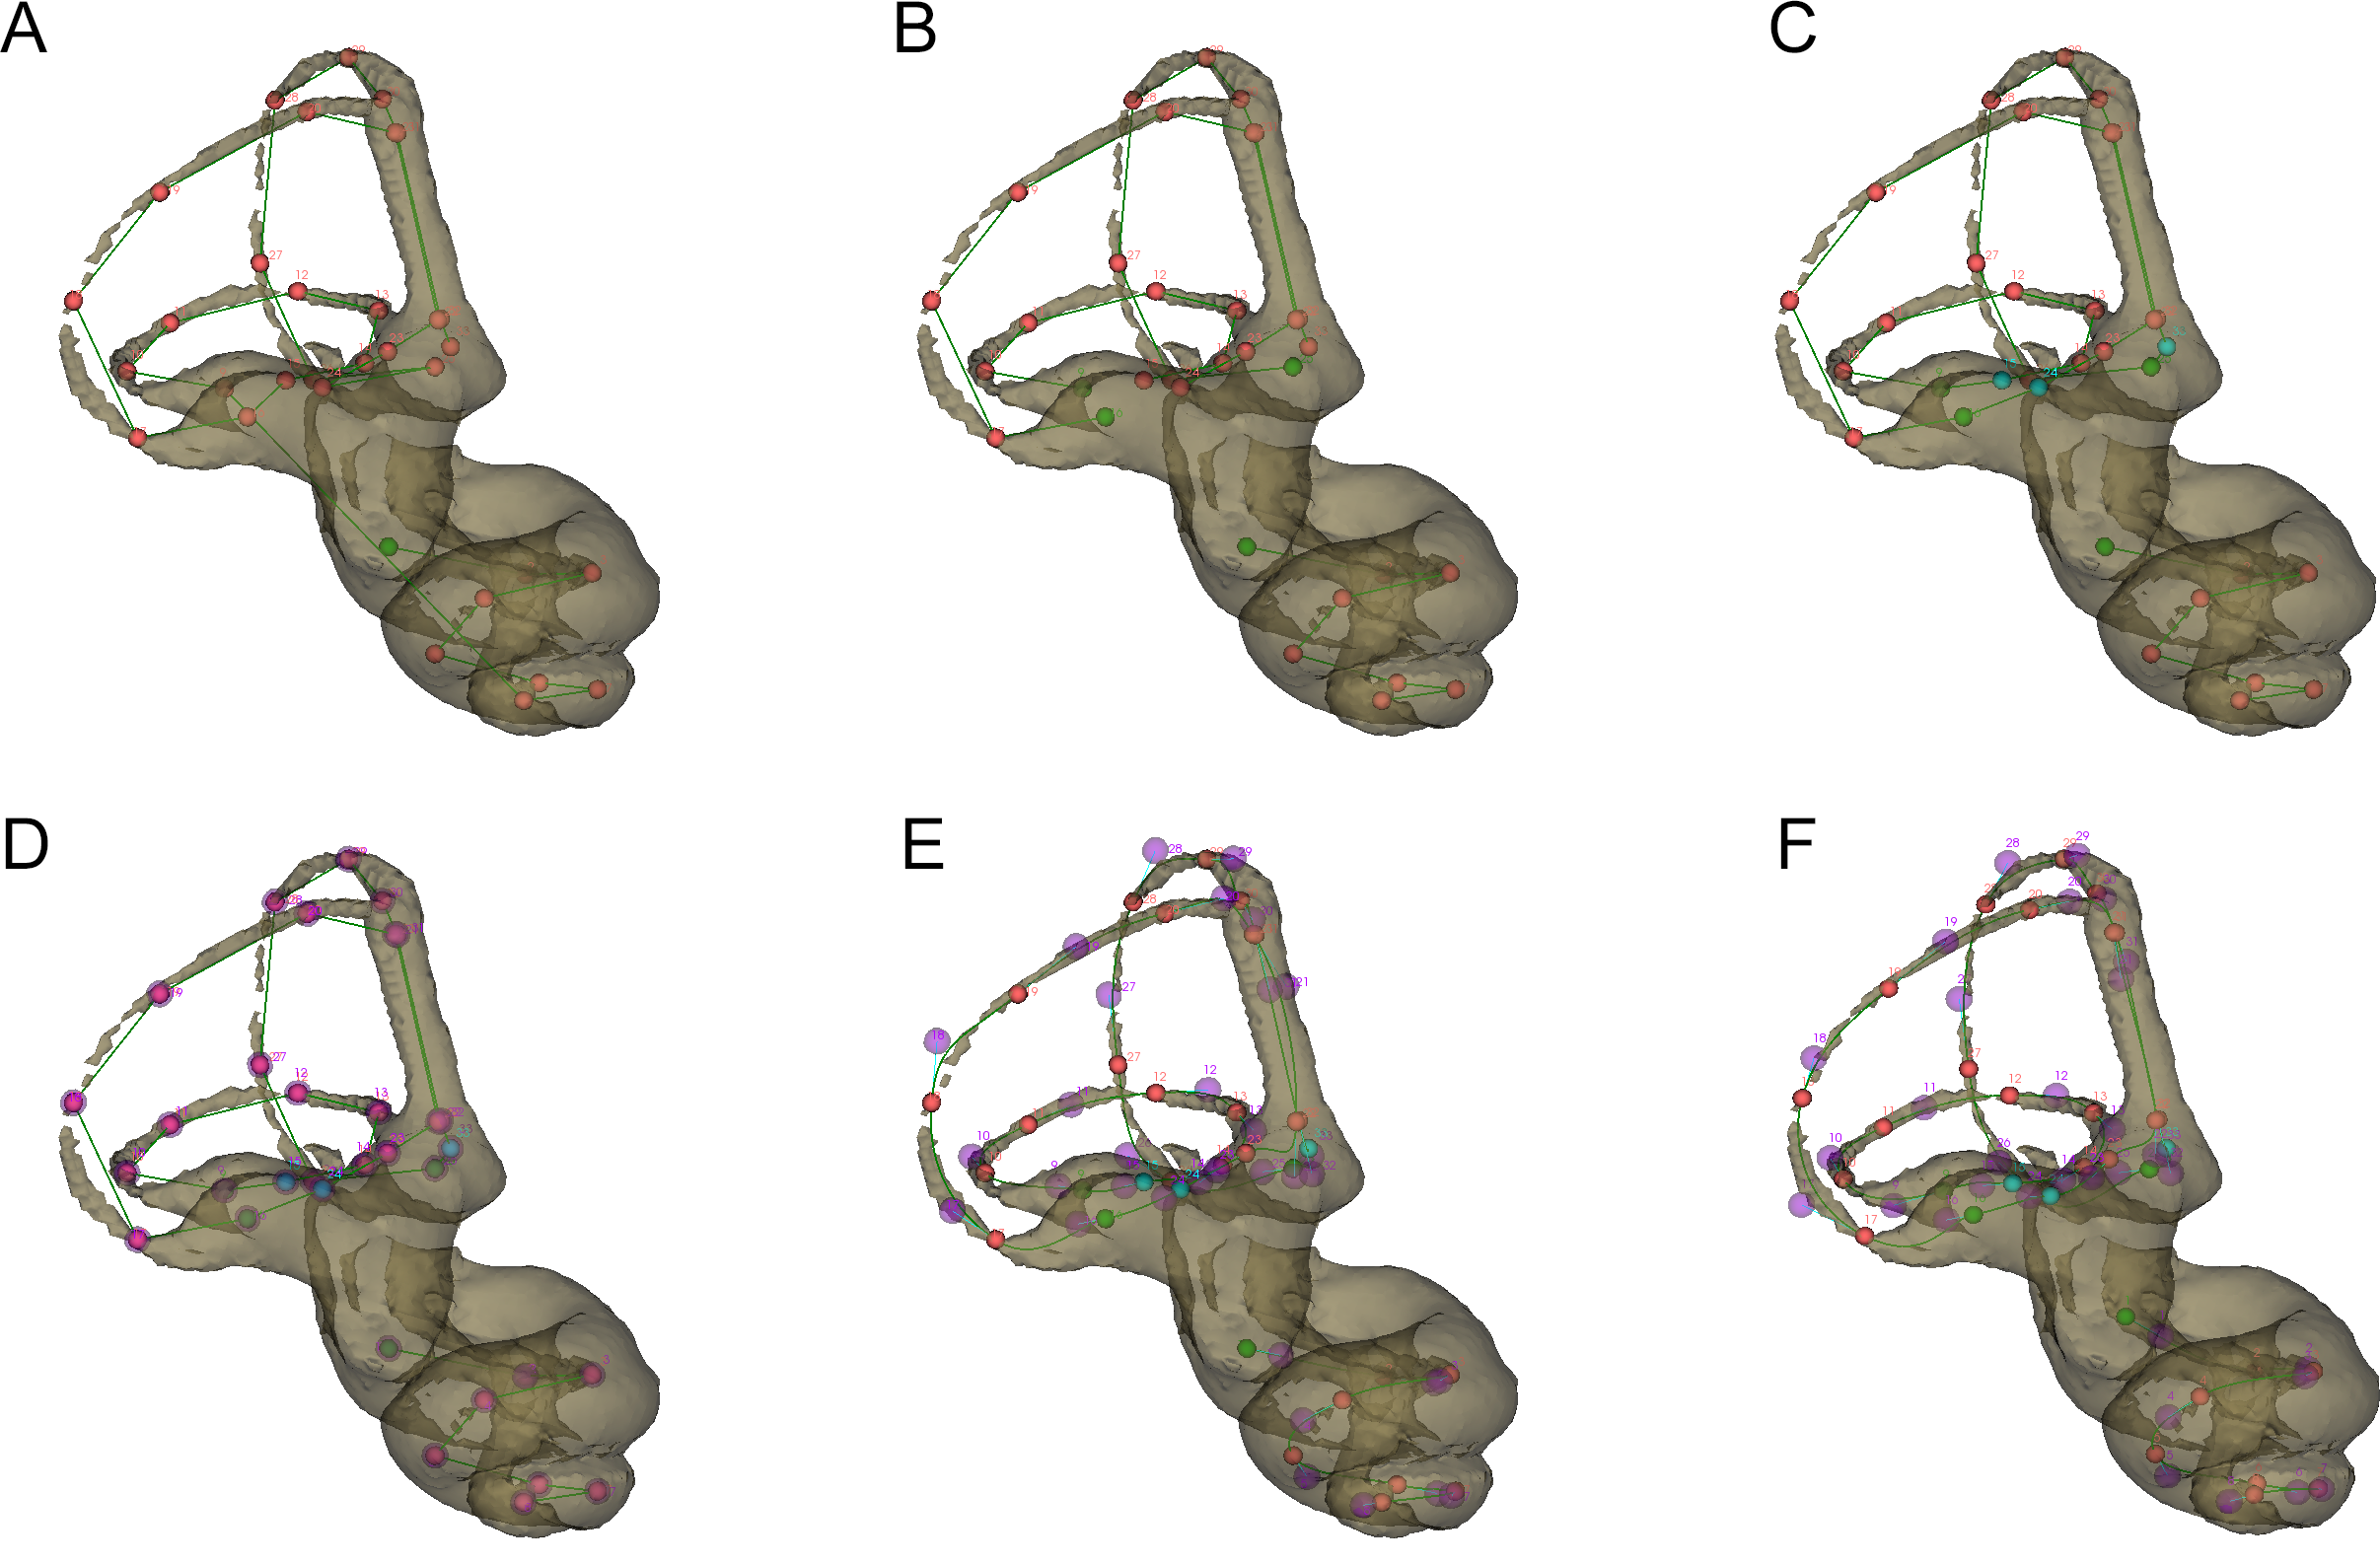
\includegraphics[scale=0.2]{curve_digitization.png} 
	\caption{Curve digitization strategy with MorphoDig. \textbf{A:} digitization of curve node landmarks. \textbf{B:} Nodes 9, 16 and 25 are now starting nodes (dark green). \textbf{C:} Nodes nodes 15, 24 and 33 are connected to their preceding starting node to close the three semicircular canals. \textbf{D:} Curve node coordinates were saved  as a .ver file, and are loaded in a second step as handle landmarks (violet). \textbf{E:} Curve handles were displaced automatically. \textbf{F:} several curve nodes and curve handles were displaced manually (last and most time consuming step)}
\label{curve_digitization}
 \end{figure}
To digitize curves on an inner ear, I recommend to use the following 3 steps strategy:
\subsubsection{1) Digitize a series of "curve node" landmarks, and define curve starting points}
As curves pass through curve node landmarks, these curve nodes will endorse the role of the "skeleton" of all curve segments. In the present tutorial, a series of 33 "curve node" landmarks was set inside the cochlea, the lateral semicircular canal, on the anterior and posterior semi-circular canals (Fig. \ref{curve_digitization}-A p.\pageref{curve_digitization}). You may load the enclosed .ver file (File->Curves->Open Curve Node Landmarks-> Mouse\_right\_ear.ver).\\

Then select landmarks 9, 16 and 25, and define them as curve starting points (Landmarks->Selected curve node and curve handle landmarks-> Normal nodes (red): define as starting nodes (dark green)). The consequence of this action is that the series of 33 landmarks will contain four
curves : one defining the cochlea, and one for each of the 3 semi-circular canals (Fig. \ref{curve_digitization}-B p.\pageref{curve_digitization}).\\

As an option, you may select curve nodes 15, 24 and 33 and connect them to their preceding starting
nodes (Landmarks->Selected curve node and curve handle landmarks-> Normal nodes (red): connect
to preceding starting nodes (cyan)). The consequence of this action is that the curves representing
the 3 semi-circular canals will be closed (Fig. \ref{curve_digitization}-C p.\pageref{curve_digitization}).\\
Save the current series of landmarks (File->Curves->Save Curve Node Landmarks).

\subsubsection{2) Load curve handles and modify their position semi-automatically}
- Load curve handles (File->Curve->Open Curve Handle Landmarks-> then select the file you just created
in the preceding step, here choose the "Mouse\_right\_ear.ver" file, Fig. \ref{curve_digitization}-D p.\pageref{curve_digitization}).\\
- Select all the curve handles (the easiest way to achieve this is to press “CTRL +A”, to select all currently
opened objects).\\
- Move curve handles semi-automatically (Landmarks->Selected curve node and curve handle landmarks-> Move curve handles semi-automatically). Choose a value of 25\%, press "Ok" (Fig. \ref{curve_digitization}-E p.\pageref{curve_digitization}), and then unselect all objects (CTRL+D).\\

\subsubsection{3) Modify curve handles and normal landmarks manually}
The last step (and probably the hardest one) is to move manually the curve nodes and curve handles in order to make the curves follow the geometry of the studied structures (Fig. \ref{curve_digitization}-F p.\pageref{curve_digitization}).

\subsection{Saving and exporting curves}
\begin{figure}
  \centering
  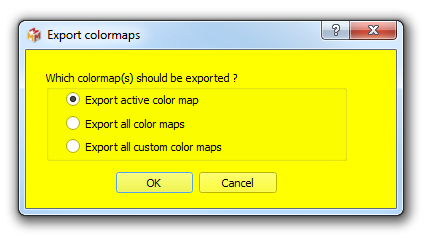
\includegraphics[scale=0.3]{export.png} 
	\caption{Exporting curves. \textbf{A:} curve digitization involving with 33 curve node and 33 curve handle landmarks. \textbf{B:} each curve segment was exported as 20 equidistant semi-landmarks inside a .ver file. These equidistant semi-landmarks are those used in geometric morphometric analyses.}
	\label{export}
 
\end{figure}
To save all digitized curves, go in “File->Curves” and either save curve nodes and curve handles inside a .STV (recommended) or .CUR file.\\ 
To export all digitized curve segments into series of equidistant semi-landmarks (these latter ones will be used in geometric morphometric analyses), go in “File->Curves->Export curves segments as landmark file” (See Fig. \ref{export} p.\pageref{export}).

\subsection{Saving the project}
Saving a "project" makes it possible to save all opened selected objects and their properties (surface of the inner ear, its transparency, color and position, curve nodes, curve handles) altogether instead of one by one. 
To save all opened objects, do the following sequence of actions:\\
1) press "CTRL + A" to select all objects\\
2) click on "File->Project->Save Project" or on the button "save project" (
\includegraphics[scale=0.03]{../images/03/save_data.png})  inside the main window.\\
3) choose the desired options in the "Save Project" window (see Fig. \ref{save_project_file} p.\pageref{save_project_file} and the User Guide for further details regarding the available options)
\begin{figure}
  \centering  
 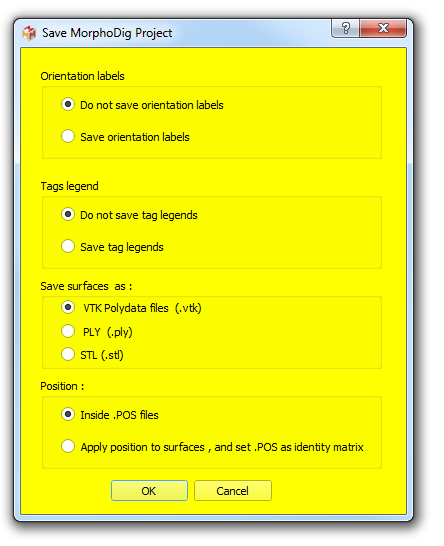
\includegraphics[scale=0.5]{../images/07/project/save_ntw.png}
 \captionof{figure}{Save project window.}
\label{save_project_file}
\end{figure}

The advantage of working with projects is that all involved objects and their properties (surfaces, landmarks, positions etc.) can be reloaded later all at once (and not 1 by 1). 

\subsection{Acknowledgements}
Thanks to the MRI imaging platform for the access to imaging facilities.

%\nocite{*}   % All bibliography items appear without citation in the text

%\cleardoublepage
%\phantomsection

%\addcontentsline{toc}{chapter}{References}
%  \bibliography{References/UsersGuide}		
\end{document} 

